\section{Methods}

The fundamental basis for the callback mechanism lies
in the C-API of the CPython interpreter. When Python code such as

\footnotesize\begin{verbatim}
results = model(*args, **kwargs)
\end{verbatim}\normalsize
is executed, it is internally translated into an equivalent C function call

\footnotesize\begin{verbatim}
PyObject *results, *model, *args, *kwargs;
PyObject *id = model;
results = PyObject_Call(id, args, kwargs);
\end{verbatim}\normalsize
This direct mapping between Python code and C function calls,
as illustrated in Figure~\ref{fig:Callback-C-API-vs-pybind11},
extends to all Python operations,
making it theoretically feasible to translate any Python code sequence
into equivalent C function calls.
While such manual translation would be impractical,
the pybind11 library \cite{Software-pybind11} substantially simplifies this process.
The implementation of the callback mechanism requires two key components:
(1) obtaining the unique identifier (a long integer) of the callable object in
Python,
which corresponds to the value of its \verb|PyObject| pointer,
achieved using Python's built-in \verb|id()| function, and
(2) transferring and storing this identifier from Python to C,
accomplished through the CPython API or binding libraries
such as pybind11 or SWIG \cite{Software-SWIG}.

After capturing the \verb|PyObject| pointer of the callable Python object
in C and ensuring that the object remains resident in memory,
model inference can proceed independently
of the ML model's deployment method or optimization strategy.
This approach establishes a robust and flexible foundation
for integrating Python-based ML models with C-based MD simulations.

\ifdefined\InlineFloatEnv
\begin{figure*}[htbp]
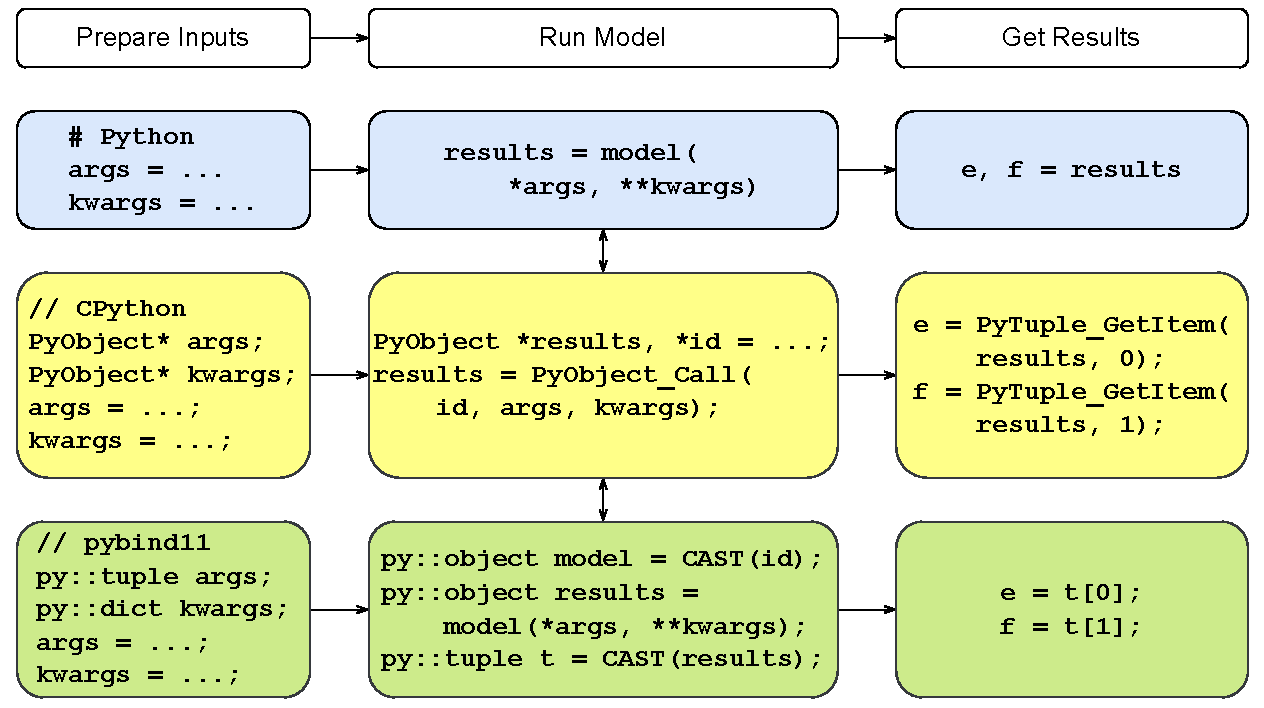
\includegraphics[width=\textwidth]{figs/Callback.pdf}
\caption{Illustration of the Python callback mechanism,
demonstrating the translation between a Python function call
and its corresponding pseudo C/C++ implementations
using either the CPython API or pybind11
(with the C++ namespace \texttt{pybind11} abbreviated
as \texttt{py}).}\label{fig:Callback-C-API-vs-pybind11}
\end{figure*}

\else\fi

The implementation is streamlined through a custom \verb|Callable| class
that encapsulates the model identifier, the return variables,
and the function parameters.
This class serves as the primary initialization parameter
for the new OpenMM force provided in the plugin.
Integration of this mechanism into an existing OpenMM Python script
is straightforward, as demonstrated below:

\footnotesize\begin{verbatim}
from CallbackPyForce import Callable, TorchForce
class Model42(torch.nn.Module):
    def forward(self, positions):
        return torch.sum(positions**2)
model42 = Model42()
model42 = torch.compile(model42)
call = Callable(id(model42), Callable.RETURN_ENERGY)
force = TorchForce(call)
openmm_system.addForce(force)
\end{verbatim}\normalsize
The Torch library handles force calculations through backpropagation
when the forward pass does not explicitly compute forces.
Additionally, this mechanism seamlessly supports model optimization
through PyTorch's compilation tools:
models can be enhanced with \texttt{\torchjit} or \texttt{\torchcompile}
simply by adding these statements to the existing code,
requiring minimal additional modifications.
